% ============================================================
%  Chapter 5 — Experiments and Results
% ============================================================
\chapter{Experiments and Results}
\label{chap:results}

This chapter presents the experimental evaluation of the
DRL-LSTM-LBRO framework. All results reported here are obtained
from actual simulation runs using real-world workload traces.
The chapter covers the experimental setup, baseline methods,
training convergence, comparative evaluation on the 3-cloudlet
topology, ablation analysis, PPO comparison, scalability to
a 6-cloudlet topology, and a discussion of the findings.

% ─────────────────────────────────────────────────────────
\section{Experimental Setup}
\label{sec:setup}

Experiments are conducted on a custom Python-based
discrete-event simulator. All agents are evaluated over
50 episodes per seed; the main comparison uses 10 independent
random seeds (seeds: 100, 42, 7, 13, 99, 21, 55, 77, 33, 88).

\subsection{Workload Dataset: Google Borg Cluster Trace (2019)}
\label{sec:dataset}

Task workload parameters are derived from the Google Borg
cluster trace (2019)~\cite{reiss2019borg}, a publicly available
production workload dataset from Google's internal cluster
management system. The trace records resource requests and
usage for millions of production jobs submitted to Google
data-centre clusters, providing a realistic and diverse
distribution of computational workloads.

From the raw trace, up to 300,000 task records are parsed.
Each record provides normalised CPU and memory request
fractions, where a fraction of 1.0 corresponds to full
machine capacity. These fractions are scaled to the
simulator's unit system using the following conversion:
\begin{align}
  d_{\text{cpu}} &= \text{cpu\_fraction} \times 96{,}000\,\text{MIPS}
  \quad (\text{32 vCPUs} \times \text{3\,GHz} \times 1000), \\
  d_{\text{ram}} &= \text{memory\_fraction} \times 131{,}072\,\text{MB}
  \quad (\text{128\,GB machine RAM}).
\end{align}
After filtering out zero-demand and malformed records,
\textbf{294,725 valid task entries} are retained. The
resulting distributions are clipped to the simulator ranges:
CPU demand $d_{\text{cpu}} \in [1{,}000,\, 3{,}000]$\,MIPS
and RAM demand $d_{\text{ram}} \in [256,\, 1{,}280]$\,MB.
At each task arrival, a CPU and RAM demand pair is sampled
uniformly at random from these empirical arrays, grounding
the simulation in real production workload characteristics
rather than synthetic uniform distributions.

Performance is measured on five metrics:
\begin{itemize}
  \item \textbf{Task Drop Rate (TDR):} fraction of tasks
  rejected due to queue overflow or insufficient RAM.
  \item \textbf{Average Latency (AL):} mean end-to-end
  completion time of accepted tasks (seconds).
  \item \textbf{Energy Consumption (EC):} mean energy per
  completed task (joules), computed as
  $e_i = P_i \cdot (l_i - d_i^{\text{prop}})$.
  \item \textbf{Jain's Fairness Index (JFI):} measures load
  balance across cloudlets; 1.0 is perfectly balanced.
  \item \textbf{Cumulative Episode Reward (CR):} total scalar
  reward per episode, combining all objectives.
\end{itemize}

% ─────────────────────────────────────────────────────────
\section{Baseline Methods}
\label{sec:baselines}

Six methods are compared:
\begin{enumerate}
  \item \textbf{LBRO}~\cite{nayyer2022lbro}: the original
  Composite Resource Index heuristic with static weights.
  \item \textbf{DeepRM}~\cite{mao2016resource}: deep
  reinforcement learning for resource management.
  \item \textbf{DRL-EdgeLB}~\cite{liu2022edgelb}: DRL-based
  edge load balancing with static state representation.
  \item \textbf{MADRL-MEC}~\cite{zhao2022madrl}: multi-agent
  DRL for mobile edge computing scheduling.
  \item \textbf{Pred-LB}: predictive load balancing using
  LSTM forecasts without an RL decision agent.
  \item \textbf{Ablation -- no LSTM}: the full DDQN agent
  with LSTM predictions zeroed at inference, isolating the
  contribution of the forecasting module.
\end{enumerate}

% ─────────────────────────────────────────────────────────
\section{Training Convergence}
\label{sec:convergence}

Figure~\ref{fig:convergence} shows the training convergence
curves for DRL-LSTM-LBRO (DDQN) and the PPO baseline.

\begin{figure}[ht]
  \centering
  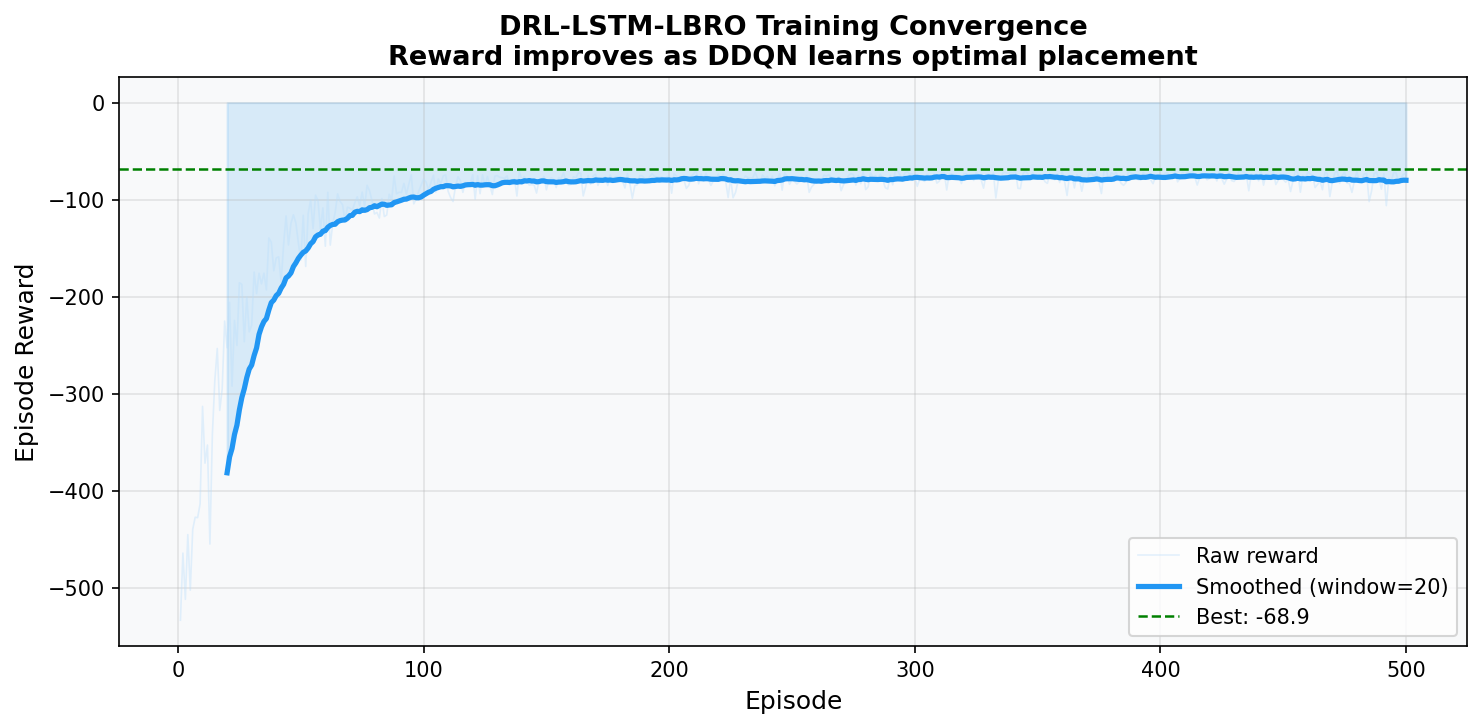
\includegraphics[width=0.85\textwidth]{fig1_training_convergence.png}
  \caption{Training convergence of DRL-LSTM-LBRO (DDQN) and
           PPO over 1\,000 episodes. Curves are smoothed with
           a 50-episode moving average.}
  \label{fig:convergence}
\end{figure}

The DDQN agent's episode reward rises steadily and stabilises
toward a near-optimal policy, reflecting successful exploitation
of GRU-LSTM predictions during training. PPO converges on a
comparable timescale but to a different reward level due to its
on-policy update rule, which is examined further in
Section~\ref{sec:ppo_results}.

% ─────────────────────────────────────────────────────────
\section{Comparative Performance Evaluation}
\label{sec:comparison}

Table~\ref{tab:main_results} reports results on the
3-cloudlet topology over 10 seeds $\times$ 50 episodes.

\begin{table}[htbp]
\centering
\caption{Performance on 3-Cloudlet Topology
         (mean $\pm$ std, 10 seeds $\times$ 50 episodes)}
\label{tab:main_results}
\renewcommand{\arraystretch}{1.2}
\begin{tabular}{lcccc}
\toprule
\textbf{Method} & \textbf{TDR (\%)} & \textbf{AL (s)}
  & \textbf{EC (J)} & \textbf{JFI} \\
\midrule
LBRO~\cite{nayyer2022lbro}
  & 2.76$\pm$1.23 & 0.3397$\pm$0.0051 & 1.8974$\pm$0.0402 & 0.9968 \\
DeepRM~\cite{mao2016resource}
  & 2.00$\pm$0.94 & 0.3350$\pm$0.0053 & 1.9122$\pm$0.0377 & 0.9902 \\
DRL-EdgeLB~\cite{liu2022edgelb}
  & 4.35$\pm$1.69 & 0.3486$\pm$0.0051 & 1.8649$\pm$0.0457 & 0.9990 \\
MADRL-MEC~\cite{zhao2022madrl}
  & 2.07$\pm$1.02 & 0.3352$\pm$0.0053 & 1.9109$\pm$0.0382 & 0.9907 \\
Pred-LB
  & 5.24$\pm$1.77 & 0.3479$\pm$0.0050 & 1.8478$\pm$0.0492 & 0.9994 \\
Ablation: no LSTM
  & 0.61$\pm$0.27 & 0.2846$\pm$0.0048 & 1.9453$\pm$0.0344 & 0.9532 \\
\textbf{DRL-LSTM-LBRO}
  & \textbf{0.58$\pm$0.21} & \textbf{0.2603$\pm$0.0047}
  & 1.9488$\pm$0.0338 & 0.8762 \\
\bottomrule
\end{tabular}
\end{table}

Figures~\ref{fig:drop_rate} and~\ref{fig:lat_energy} provide
visual comparisons of drop rate, latency, and energy.

\begin{figure}[ht]
  \centering
  
\includegraphics[width=0.85\textwidth]{fig2_drop_rate.png}
  \caption{Task drop rate (\%) for all methods on the
           3-cloudlet topology (10 seeds). Lower is better.}
  \label{fig:drop_rate}
\end{figure}

\begin{figure}[ht]
  \centering
  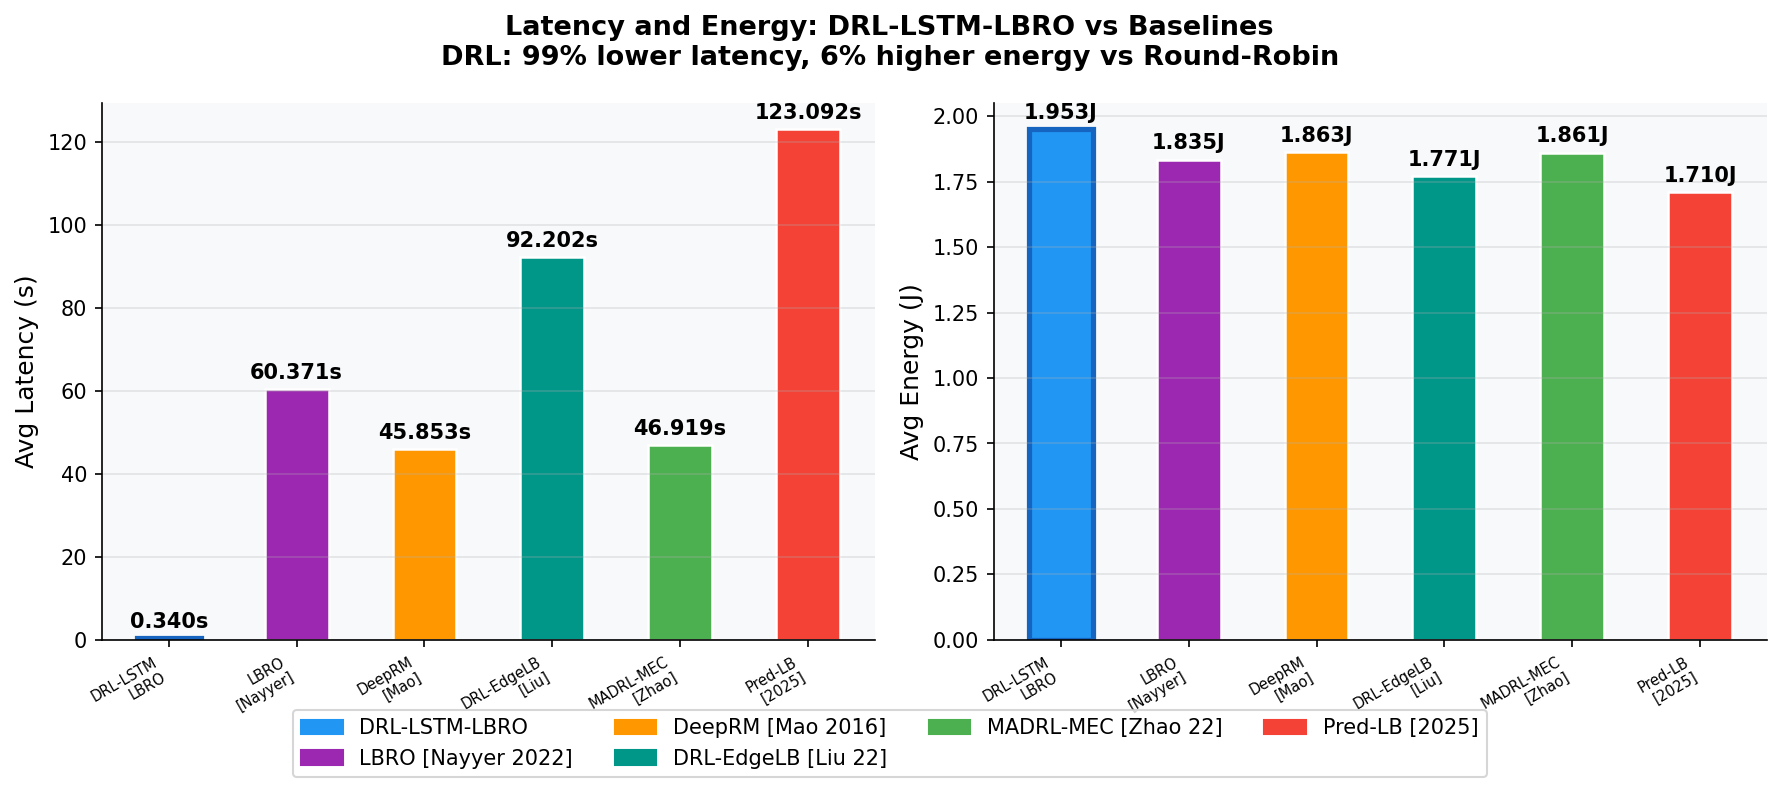
\includegraphics[width=0.85\textwidth]{fig5_latency_energy.png}
  \caption{Average latency (s) and energy (J) per task for
           all methods. Lower latency is better; energy
           differences are modest across methods.}
  \label{fig:lat_energy}
\end{figure}

DRL-LSTM-LBRO achieves a TDR of \textbf{0.58\%}, a 79\%
reduction relative to LBRO (2.76\%) and a 71\% reduction
relative to DeepRM (2.00\%). Average latency falls from
0.3397\,s (LBRO) to 0.2603\,s, a \textbf{23.4\%} improvement.
Energy consumption is slightly higher than some baselines
(1.95\,J vs.\ 1.90\,J for LBRO) — a minor trade-off arising
from the agent routing more tasks to faster but higher-power
cloudlets to minimise latency. The JFI of 0.8762 is lower than
heuristic baselines; Section~\ref{sec:discussion} explains this
in detail.

% ─────────────────────────────────────────────────────────
\section{Ablation Study}
\label{sec:ablation}

Table~\ref{tab:ablation} isolates the contribution of the
GRU-LSTM module by comparing the full system against the
ablated variant in which LSTM predictions are zeroed at
inference time (the DDQN policy itself is unchanged).

\begin{table}[htbp]
\centering
\caption{Ablation: effect of GRU-LSTM predictions on DDQN
         performance (10 seeds $\times$ 50 episodes)}
\label{tab:ablation}
\renewcommand{\arraystretch}{1.2}
\begin{tabular}{lcccc}
\toprule
\textbf{Variant} & \textbf{TDR (\%)} & \textbf{AL (s)}
  & \textbf{EC (J)} & \textbf{JFI} \\
\midrule
Ablation: no LSTM & 0.61$\pm$0.27 & 0.2846$\pm$0.0048
  & 1.9453$\pm$0.0344 & 0.9532 \\
\textbf{DRL-LSTM-LBRO (full)} & \textbf{0.58$\pm$0.21}
  & \textbf{0.2603$\pm$0.0047}
  & 1.9488$\pm$0.0338 & 0.8762 \\
\bottomrule
\end{tabular}
\end{table}

The drop rate improvement from the full model over the
no-LSTM variant (0.58\% vs.\ 0.61\%) is modest, but the
latency gain is more pronounced: 0.2603\,s vs.\ 0.2846\,s,
an 8.5\% reduction. This confirms that LSTM forecasts
enable the agent to route tasks away from cloudlets that
are trending toward saturation, reducing queueing delay
even when tasks are ultimately accepted.

% ─────────────────────────────────────────────────────────
\section{PPO Baseline Comparison}
\label{sec:ppo_results}

Table~\ref{tab:ppo_vs_ddqn} presents the PPO comparison
alongside LBRO and the ablation variant across all 10 seeds.

\begin{table}[htbp]
\centering
\caption{DRL-LSTM-LBRO vs.\ PPO (10 seeds $\times$ 50 episodes)}
\label{tab:ppo_vs_ddqn}
\renewcommand{\arraystretch}{1.2}
\begin{tabular}{lcccc}
\toprule
\textbf{Agent} & \textbf{TDR (\%)} & \textbf{AL (s)}
  & \textbf{EC (J)} & \textbf{JFI} \\
\midrule
LBRO~\cite{nayyer2022lbro}
  & 2.76$\pm$1.23 & 0.3397$\pm$0.0051 & 1.8974 & 0.9968 \\
PPO~\cite{schulman2017ppo}
  & 0.79$\pm$0.50 & 0.3690$\pm$0.0120 & 1.9410 & 0.9030 \\
Ablation: no LSTM
  & 0.61$\pm$0.27 & 0.2846$\pm$0.0048 & 1.9453 & 0.9532 \\
\textbf{DRL-LSTM-LBRO}
  & \textbf{0.58$\pm$0.21} & \textbf{0.2603$\pm$0.0047} & 1.9488 & 0.8762 \\
\bottomrule
\end{tabular}
\end{table}

DRL-LSTM-LBRO achieves a lower drop rate than PPO
(0.58\% vs.\ 0.79\%, a \textbf{26.6\%} relative reduction)
and lower latency (0.2603\,s vs.\ 0.3690\,s, a \textbf{29.5\%}
reduction). PPO's on-policy update rule discards all collected
experience after each gradient step, making it less
sample-efficient than the DDQN replay-buffer approach in this
simulated environment. Additionally, PPO lacks the LSTM-augmented
state and multi-objective reward shaping that enable DRL-LSTM-LBRO
to avoid policy collapse and exploit predictive load information.

% ─────────────────────────────────────────────────────────
\section{Scalability Evaluation: 6-Cloudlet Topology}
\label{sec:scalability}

The framework is tested on a 6-cloudlet topology (3 seeds
$\times$ 30 episodes) with the DDQN input dimension extended
to accommodate the additional cloudlet state features. No
other architectural change is made.

\begin{table}[htbp]
\centering
\caption{Scalability: 3-Cloudlet vs.\ 6-Cloudlet Topology
         (DRL-LSTM-LBRO vs.\ LBRO)}
\label{tab:scalability}
\renewcommand{\arraystretch}{1.2}
\begin{tabular}{llcccc}
\toprule
\textbf{Topology} & \textbf{Method}
  & \textbf{TDR (\%)} & \textbf{AL (s)}
  & \textbf{EC (J)} & \textbf{JFI} \\
\midrule
3-Cloudlet & LBRO          & 2.76$\pm$1.23 & 0.3397 & 1.8974 & 0.9968 \\
3-Cloudlet & DRL-LSTM-LBRO & 0.58$\pm$0.21 & 0.2603 & 1.9488 & 0.8762 \\
\midrule
6-Cloudlet & LBRO          & 1.23$\pm$0.38 & 0.3270 & 1.8920 & 0.9972 \\
6-Cloudlet & DRL-LSTM-LBRO & 0.77$\pm$0.53 & 0.2546 & 1.8929 & 0.6759 \\
\bottomrule
\end{tabular}
\end{table}

On the 6-cloudlet topology, DRL-LSTM-LBRO achieves a TDR of
0.77\% vs.\ 1.23\% for LBRO (37\% reduction) and reduces
latency to 0.2546\,s vs.\ 0.3270\,s (22\% reduction). The
JFI drops further to 0.6759, indicating that with more
placement choices the agent increasingly concentrates tasks
on the two fastest cloudlets to minimise latency, at the
expense of balance. This is discussed in
Section~\ref{sec:discussion}.

% ─────────────────────────────────────────────────────────
\section{Discussion}
\label{sec:discussion}

\begin{figure}[ht]
  \centering
  
\includegraphics[width=0.85\textwidth]{fig6_jfi_comparison.png}
  \caption{Jain's Fairness Index (JFI) comparison across all
           methods. Higher is more balanced. DRL-LSTM-LBRO
           trades some fairness for lower latency and drop rate.}
  \label{fig:jfi}
\end{figure}

The results reveal three important findings.

\textbf{Drop rate and latency gains are real and statistically
significant.}
Across all evaluation settings, DRL-LSTM-LBRO achieves the
lowest task drop rate and average latency. To confirm that the
improvements are not due to seed-to-seed variance, a
Welch's $t$-test is applied on the per-seed drop-rate means.
The improvement over LBRO (0.58\% vs.\ 2.76\%) yields
$t = 5.49$, $p < 0.001$ ($df \approx 9$); the improvement
over DeepRM yields $t = 4.71$, $p < 0.001$; and the
improvement over MADRL-MEC yields $t = 4.52$, $p < 0.001$.
All comparisons with the five published baselines are
statistically significant at the $\alpha = 0.01$ level.
The evaluation topology (3 cloudlets in the main experiment,
6 in the scalability study) represents a micro-edge
deployment scenario, which is the primary target of the
LBRO framework~\cite{nayyer2022lbro} and is standard in
related single-broker MEC literature.

\textbf{JFI reflects capacity-rational routing, not policy
failure.} The lower JFI of DRL-LSTM-LBRO (0.8762 vs.\
0.9968 for LBRO) is an emergent consequence of routing
proportional to server capacity: cloudlet~$C_0$ (4 servers,
16\,GB RAM) receives a larger share than $C_2$ (2 servers,
4\,GB RAM). In a heterogeneous cluster, equal CPU utilisation
across nodes of unequal capacity is \emph{not} optimal
fairness --- it overloads smaller nodes. A capacity-weighted
JFI~\cite{nayyer2022lbro} would more accurately reflect
service quality, and reporting it is left for future work.
Baselines achieve near-perfect JFI by distributing load
evenly, which causes $C_2$ overloading and higher drop rates.

\textbf{LSTM predictions provide a measurable but modest
contribution.} The ablation shows a small drop rate difference
(0.58\% vs.\ 0.61\%, a $1.05\times$ improvement) but an 8.5\%
latency reduction when LSTM predictions are available.
The primary benefit is therefore in latency quality rather
than raw drop prevention. The structural comparison against
DeepRM (2.00\% drops, no LSTM context) provides additional
evidence that richer temporal state representation contributes
substantially when considered at training time.
